\subsubsection{Description Processing}
\par As the movie description was provided was in German, we first used Google
Translate to translate the description to English before proceeding with 
any further processing. Though there may be translational errors, it was decided that it was best to transform the original descriptions (versus using other English descriptions) to maintain the original time stamps from the researchers to have optimal alignment between the description and FMRI data.

\par Due to grammatical differences, we decided to only keep nouns and verbs, and discarded the adjectives and other words including stop-words, which are commonly used words with little meaning or determinable context (e.g. 'and', 'to', 'him'). A publicly available list of stop-words from Princeton University was used for this task, and iteratively appended to until our determined set of words contained no blatantly uninformative words. Of the words that remained, a WordNet dictionary was built, which is a popular way to tag words according to a context-specific definition, and classify them based on hierarchical similarities, eventually grouping English words into sets of synonyms called synsets. In this way, words as stand-alone entities will have an unambiguous definition and deeper relationships can be derived from the correlations found. 

 \par Word categories are determinable through WordNet, which classifies words based on hierarchical similarities and assigns semantic labels to distinguish between homophones, grouping English words into sets of synonyms called synsets.  
 \par After aggregating the set of all contextual definitions of words,
 we build a design matrix composed of the descriptive entries in the movie description. Thus each interval of time with a sentence description of the movie events was treated as a row, and each column represented a context-specific word as a feature. The matrix values are all binary, with a value of '1' indicating that the word is present at that time, while '0' indicates that it is not. This was illustrated as a rectangular image with a white square for '1' and black for '0'. 

\begin{figure}[!htbp]
\centering
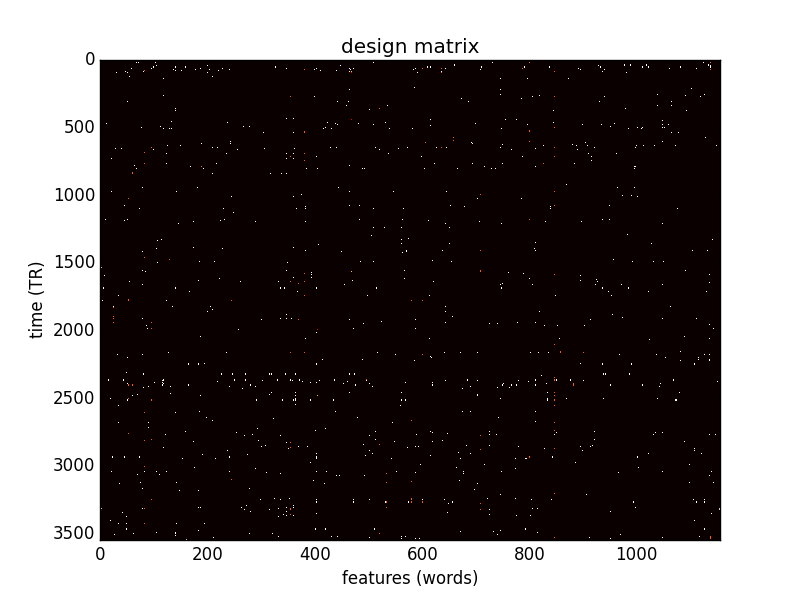
\includegraphics[width=0.5\textwidth]{design_matrix.png}
\caption{\label{fig:design_matrix} A visualization of design matrix for the semantic modeling}
\end{figure}

Finally, in order to format the data such that it correlates explicitly
to the FMRI images, the intervals were split into two-second intervals
to create a one-to-one representation between description objects and images. As can be seen in Figure 1 above, this matrix is quite sparse, as many words often appear for only a few seconds in the duration of the movie. 

\subsubsection{Scenes Processing}
\par The provided scenes file includes the start and end times of each of the 90 distinct movie scenes. We converted the scenes file into a csv (saved as 'scenes num times.csv' in the data folder) containing four columns: onset time, duration, amplitude, and factor id. The first time starts at 17 seconds because of credits, and most of the 90 distinct categories are very similar. For example, "Gump House" is in a separate category as "Gump Bedroom". Moreover, many scenes only occur once and only for a small fraction of time. Because of these similarities, we created the following scene categories: "Gump", "Military", "School", "Savanna", "Outside", and "Political". While these categories do not include every scene, they capture most of the scenes in the movie. For a more detailed list of the specific scenes that comprise each category, please look at 'scenes pred' script in the code folder.  